\chapter{The mathematical theory of symmetries}

In this chapter, the mathematical theory used in the thesis will be presented.
The theory mostly concerns symmetry groups in the setting of ordinary differential equations (ODE:s), and systems thereof.
To aid readers new to this subject and with varying familiarity with related mathematical subjects, the theory is presented in a straight forward fashion, avoiding unnecessary generalizations and proofs of most results.
The mathematical theory and notation used in this and subsequent chapters is based on the works of three authors.
For readers wishing to explore the subject further, the sources are presented here in short.

The first source \cite{hydon2000symmetry} by \citeauthor{hydon2000symmetry}, serves as a great introductory text on the subject of symmetry methods.
For readers unfamiliar with the fields of differential geometry and Lie algebras wishing to use methods similar to the ones in this thesis, the book can be helpful for getting off the ground.
This is mainly due to fact that theory is only introduced on a need to know basis throughout the book, and as such readers seeking the mathematical rigor lacking in this text will not find it there.

The second sources \cite{olver1993applications,olver1995equivalence} by \citeauthor{olver1993applications}, on the other hand treats the subject stringently and serves as good reference points for readers wishing to understand the theory in more depth.
While \cite{olver1993applications} focuses more on the specific application to differential equations, \cite{olver1995equivalence} puts more focus on the geometric concepts involved.

The third source \cite{ovsiannikov1982group} by \citeauthor{ovsiannikov1982group}, deals with group classification, a slightly more advanced subject on which the technique developed in \cref{ch:param-ind} is based. % TODO: Maybe elaborate on group classification
Due to its earlier publication date, the book treats some subjects in a less modern way than the works by \citeauthor{hydon2000symmetry} and \citeauthor{olver1993applications}, and is therefore not recommended for readers unfamiliar with the concerned theory.

The notation in this thesis will be based on the notation in \cite{hydon2000symmetry}, employing partial notational concepts from \cite{olver1995equivalence} and \cite{ovsiannikov1982group} when further clarity is desired.

%=============================================================================
\section{Point symmetries}

In mathematics, a symmetry is a transformation that preserves some structure.
The word symmetry is used since the mathematical concept of symmetry encompasses what is meant by symmetry in everyday speech.
A symmetric face is a face such that when mirrored it looks the same.
Here, mirroring is the transformation and \enquote{looking the same} is the structure.
In mathematics, however, the structure must be well defined, or in more common language must be a statement that has a clear distinction between being true or false.
The transformation can also be chosen more freely, beyond the transformations usually implied when talking about symmetries in everyday speech.

The most common example of a mathematical symmetry is rotating and flipping a triangle.
The structure of the triangle can be stated as the location of all the vertices and the length of the edges between specific vertices.
Rotating an equilateral triangle 120 or 240 degrees around its center, as seen in \cref{fig:triangle-rotation}, will change the location of each individual vertex, but the positions of the set of all vertices will remain the same.
Since the edges are unchanged relative to the points, these rotations constitute a symmetry of the triangle.
It is worth noting that the rotational transformations map points from the 2-dimensional plane to the two dimensional plane or, stated in mathematical terms, the rotations are mappings \(\Gamma: \reals^2 \to \reals^2\).
\begin{figure}
  \centering
  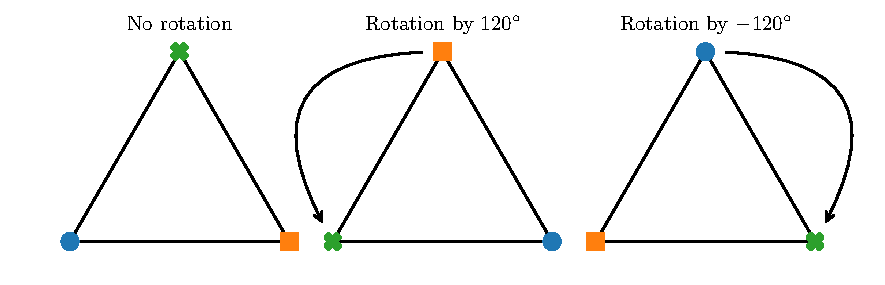
\includegraphics[width=.96\textwidth]{images/triangles}
  \caption{Rotational symmetries of an equilateral triangle.}
  \label{fig:triangle-rotation}
\end{figure}

In the methods used in this thesis, transformations similar to such a \(\Gamma\) are considered, but the structure of a triangle is instead replaced with the structure of a differential equation.
Initially, assume the differential equation is an ODE of the first order and can thus be written on the form
\begin{equation} \label[ode]{eq:first-order-ode}
  \diff{y}{x} = \omega(x,y).
\end{equation}
The structure of a first order ODE is thus defined by the function \(\omega\).
\(\omega\) is hence related to an infinite set of solutions \(u(x)\) that all fulfill \cref{eq:first-order-ode}.
Geometrically, a solution (or any scalar function of \(x\) for that matter) can be thought of as a set \(\gamma_u\) of points in the \(xy\)-plane, which constitutes a curve, for which \(y = u(x)\) holds for all \(x\).
Not every curve in the \(xy\)-plane corresponds to a function however.
A curve corresponds to a function if and only if it is transverse to the \(y\)-axis, that is: the tangent of the curve never points in only the \(y\)-direction.
Additionally for a given ODE, every point in the \(xy\)-plane belongs to exactly one such curve \(\gamma_u\): the curve of the solution that runs through that point.

A symmetry of a first order ODE \labelcref{eq:first-order-ode} is a transformation that preserves the solution curves.
This means that if two points \(\left(x_1,y_1\right)\) and \(\left(x_2,y_2\right)\) belong to the same solution curve \(\gamma\), the transformed points \(\Gamma(x_1,y_1)\) and \(\Gamma(x_2,y_2)\) must belong to the same solution curve, denoted by \(\Gamma\gamma\), for the transformation \(\Gamma\) to be a symmetry.
This property can be defined as:
\begin{defn}[Point symmetry] \label{defn:first-order-symmetry}
  A transformation 
  \begin{equation*}
    \Gamma: \left(x,y\right) \mapsto \left(\hat{x}(x,y), \hat{y}(x,y)\right)
  \end{equation*}
  is a point symmetry of \cref{eq:first-order-ode} if
  \begin{equation*}
    \diff{y}{x} = \omega(x,y)
    \implies
    \diff{\hat{y}}{\hat{x}} = \omega(\hat{x},\hat{y}).
  \end{equation*}
\end{defn}
The \enquote{point} in the term \enquote{point symmetry} refers to the fact that the transformation \(\Gamma\) only acts on the points belonging to the solution curves and nothing else.
This must not always be the case when generalizing the theory, but those generalizations will not be touched upon in this thesis.

%-----------------------------------------------------------------------------
\subsection{Jet spaces} \label{subsec:jet-spaces}

The observant reader might have already noted that there is some need for clarification of \cref{defn:first-order-symmetry}.
While the transformation \(\Gamma\) treats \(y\) as a point in \(\reals\), \cref{eq:first-order-ode} treats \(y\) as a differentiable function of \(x\), or in other words an element \(y(x)\) of the set of once continuously differentiable functions \(\mathcal{C}^1(\reals)\).
In many contexts this abuse of notation could be accepted without further remarks, but when using symmetry methods the subtleties of this operation is key to the calculations performed.
To avoid confusion while introducing the subject in this subsection, the point representation will be denoted by \(y\) while the function representation will be denoted by \(f(x)\).

The \(xy\)-plane previously mentioned can be seen as consisting of two components: the space of independent variables \(B \simeq \reals\), also known as the base space, and the space of dependent variables \(F \simeq \reals\), also known as the fiber.
The plane then is the product space \(E = B \times F \simeq \reals^2\).
It is in this plane \(E\), commonly called the total space, that the curves \(\gamma\) live.
To be able to formulate first order differential statements, the space \(F_1 \simeq \reals\) is used.
The elements of \(F_1\) will be denoted \(y'\) or \(y^{(1)}\), implying that the elements correspond to the first derivative \(f'(x)\) of the function \(f(x)\).
It is however important to note that \(F_1\) is no more the space of derivative functions \(f'(x)\) than \(F\) is the space of once continuously differentiable functions \(f(x)\); the implied relation between the two is merely aesthetic so far.
Together with the fiber \(F\), \(F_1\) forms the prolonged fiber \(\prolong{F}{1} = F \times F_1\).
The prolonged fiber \(\prolong{F}{1}\) can be combined with the base space \(B\) to create \(J_1 = J_1 E = E \times F_1 = B \times \prolong{F}{1} \simeq \reals^3\), the first order jet space of \(E\).

All differentiable functions \(f: B \to F\) have a unique equivalent function \(\prolong{f}{1}: B \to \prolong{F}{1}\) called the first prolongation of \(f(x)\), defined as
\begin{equation*}
  \prolong{f}{1}(x) = \left(f(x), \diff{f}{x}(x)\right).
\end{equation*}
In extension to this concept, a smooth transverse curve \(\gamma \subset E\) has a prolongation which is a curve \(\prolong{\gamma}{1} \subset J_1\) defined by
\begin{equation*}
  \prolong{\gamma}{1} = \left\{\left(x, \prolong{f}{1}(x)\right): x \in B\right\},
\end{equation*}
where \(f\) is the function corresponding to the curve \(\gamma\).

Using these tools, \cref{eq:first-order-ode} can be reformulated using jet spaces.
The purpose of the ODE is to define some set of solutions, and as such the reformulation should define that same set of solutions.
Using jet-notation, the problem can be formulated as finding curves \(\prolong{\gamma}{1}\) in \(J_1\) satisfying
\begin{equation} \label{eq:first-order-jet-ode}
  \Delta(\prolong{z}{1}) := y' - \omega(x,y) = 0,
\end{equation}
as well as the condition that the curve is a prolongation of some curve \(\gamma\) corresponding to a continuously differentiable function.
The curves \(\gamma\) will then correspond to the solutions \(u(x)\) of \cref{eq:first-order-ode}.
This can be seen in \cref{fig:jet-surface}, where the prolongations of the solution curves lies on the jet-surface defined by \cref{eq:first-order-jet-ode}.
\begin{figure}
  \centering
  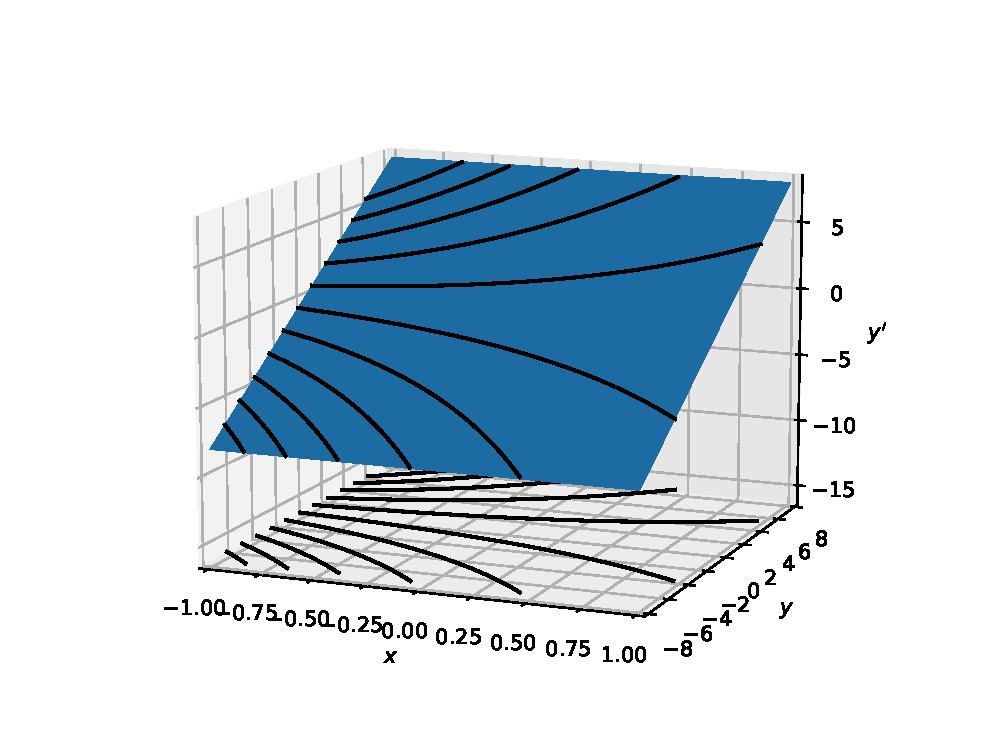
\includegraphics[width=.75\textwidth]{images/jet-surface}
  \caption{The surface \(y' = y\), and solution curves to the corresponding differential equation both prolonged to the jet space and projected on the \(x\)-\(y\)-plane.}
  \label{fig:jet-surface}
\end{figure}

While only first order ODE:s are handled in this thesis, some basic knowledge of symmetry methods for higher order ODE:s is required to be able to understand how the process of finding symmetries differ between first and higher order ODE:s.
An ODE of degree \(k\) can be written on the form
\begin{equation*}
  \diff[k]{y}{x} = \omega\left(x, y, \diff{y}{x}, \dots, \diff[k-1]{y}{x}\right),
\end{equation*}
while higher order jet spaces \(J_k = J_k E\) take the form
\begin{equation*}
  J_k = B \times F \times F_1 \times \dots \times F_k
\end{equation*}
with elements
\begin{equation*}
  \prolong{z}{k} = \left(x, y, y', \dots, y^{(k)}\right).
\end{equation*}
An ODE of degree \(k\) can thus be formulated as finding curves in \(J_k\) that satisfy
\begin{equation*}
  \Delta(\prolong{z}{k}) = y^{(k)} - \omega(x, y, y', \dots, y^{(k-1)}) = 0
\end{equation*}
as well as the condition that the curves should be \(k\):th order prolongations
\begin{equation*}
  \prolong{\gamma_u}{k} = \left\{\prolong{z}{k} = \left(\fixed{x}, y, y', \dots, y^{(k)}\right):\quad y^{(l)} = \diff[l]{u}{x}{(\fixed{x})},\quad \fixed{x} \in B,\quad l = 0, \dots, k\right\}
\end{equation*}
of curves \(\gamma\) corresponding to functions \(u(x) \in \cont{k}{B}\).
Here \(y^{(0)} = y\) and \(\diff[0]{u}{x} = u(x)\).

%-----------------------------------------------------------------------------
\subsection{The total derivative}

Since the jet space \(J_k\) treats the variables \(y\), \(y'\), \dots, \(y^{(k)}\) as independent coordinates, differentiation in \(x\), denoted as \(\partial_x\), will not affect those terms.
While this is the desired behavior of a jet space, there is also a need to be able to mirror the behavior of differentiation of the functions \(y(x)\), \(y'(x)\), \dots, \(y^{(k)}(x)\) in \(x\).
Thus a differential operator
\begin{equation*}
  \tD{x} = \partial_x + y' \cdot \partial_y + y'' \cdot \partial_{y'} + \dots + y^{(k+1)} \cdot \partial_{y^{(k)}}
\end{equation*}
on \(J_k\) is introduced, called the total derivative.
\(\tD{x}\) will act on expressions in \(J_k\) in the same way that \(\diff*{}{x}\) would act on corresponding expressions consisting of \(x\), \(y(x)\) and derivatives of \(y(x)\) in \(x\).

A change of variables
\begin{align*}
  \hat{x} &= \hat{x}(x, y(x))\\
  \hat{y} &= \hat{y}(x, y(x)) = \hat{y}(\hat{x})
\end{align*}
in the function space can be represented in the jet space using the total derivative.
Due to the chain rule,
\begin{equation*}
  \diff{\hat{y}}{\hat{x}} = 
  \frac{\diffp{\hat{y}}{x} + \diffp{\hat{y}}{y} \diff{y}{x}}{\diffp{\hat{x}}{x} + \diffp{\hat{x}}{y} \diff{y}{x}}
\end{equation*}
in the function space.
In order to keep the correspondence between the function view and the jet view, viewing the change of variables as a transformation
\begin{equation*}
  \Gamma: \left(x,y\right) \mapsto \left(\hat{x}(x,y), \hat{y}(x,y)\right),
\end{equation*}
the first prolongation of that transformation defined by
\begin{equation*}
  \prolong{\Gamma}{1}: \left(x,y,y'\right) \mapsto \left(\hat{x}(x,y), \hat{y}(x,y), \frac{\tD{x} \hat{y}(x,y)}{\tD{x} \hat{x}(x,y)}\right)
\end{equation*}
will retain the correspondence to the ODE in the changed variables.

Using the prolongation of the transformation, \cref{defn:first-order-symmetry} of a first order symmetry for \cref{eq:first-order-ode} can be restated in the first order jet space \(J_1\) for the corresponding \cref{eq:first-order-jet-ode}.
\begin{lem} \label{lem:simple-first-order-symmetry}
  A transformation \(\Gamma: \left(x,y\right) \mapsto \left(\hat{x}(x,y), \hat{y}(x,y)\right)\) is a point symmetry of \cref{eq:first-order-ode} if and only if
  \begin{equation} \label{eq:simple-first-order-symmetry}
    \frac{\partial_x \hat{y} + \omega(x,y) \partial_y \hat{y}}{\partial_x \hat{x} + \omega(x,y) \partial_y \hat{x}} = \omega(\hat{x},\hat{y})
  \end{equation}
  holds.
\end{lem} % FIXME: Requirement of diffeomorphism
Given a transformation \(\Gamma\), it is therefore easy to check whether it is a point symmetry of \cref{eq:first-order-ode}.
The reverse process (finding point symmetries of \cref{eq:first-order-ode}) is on the other hand not easy, as \cref{eq:simple-first-order-symmetry} will in all but the most trivial cases result in a non-linear PDE in with two unknown functions.
However, by restricting attention to a specific type of point symmetries, these conditions can be simplified.

%=============================================================================
\section{Lie point symmetries}

A common restriction when studying symmetries is to limit the scope of sought symmetries to Lie groups of symmetries.
A Lie group is a mathematical group, where the members of the group can be parametrized by one or several continuous parameters. % TODO: Write footnote on groups
A Lie group of transformations on \(E\) is thus a group with composition as the operator, where the transformations are parameterized by one or several continuous parameters.
If the transformations can be indexed by a single real parameter \(\epsilon \in \reals\), the Lie group is said to be a one-parameter (real) Lie group of transformations.
The transformations in such a Lie group can be parametrized as
\begin{equation*} %\label{eq:1p-lie-point-symmetry}
  \Gamma_\epsilon: \left(x,y\right) \mapsto \left(\hat{x}_\epsilon(x,y), \hat{y}_\epsilon(x,y)\right),
\end{equation*}
where both \(\hat{x}_\epsilon(x,y)\) and \(\hat{y}_\epsilon(x,y)\) are smooth (and therefore differentiable) in \(\epsilon\) when fixing \(x\) and \(y\).
Additionally, the transformation parametrized by \(\epsilon = 0\) will be the identity transformation \(\Gamma_0: \left(x,y\right) \mapsto \left(x,y\right)\).

If all transformations in such a group are symmetries of a differential equation, the group is said to be a Lie point symmetry of the differential equation.
The following is a simple example of a one parameter Lie point symmetry.
\begin{exmp}
  The ODE
  \begin{equation} \label{eq:ex-a:ode}
    \diff{y}{x} = y = \omega(x, y)
  \end{equation}
  has several symmetries.
  One group of symmetries is
  \begin{equation} \label{eq:ex-a:transformation}
    \Gamma_\epsilon(x,y) =
    \left(\hat{x}_\epsilon(x,y), \hat{y}_\epsilon(x,y)\right) =
    \left(x + \epsilon, y\right), \quad
    \forall \epsilon \in \reals
  \end{equation}
  This can be shown by considering \cref{eq:ex-a:ode} in the jet space \(J_1\), resulting in
  \begin{equation*}
    \frac{\partial_x \hat{y}_\epsilon + \omega(x,y) \partial_y \hat{y}_\epsilon}{\partial_x \hat{x}_\epsilon + \omega(x,y) \partial_y \hat{x}_\epsilon} =
    \frac{y}{1} =
    \hat{y}_\epsilon =
    \omega(\hat{x}_\epsilon,\hat{y}_\epsilon), \quad
    \forall \epsilon \in \reals.
  \end{equation*}
  So by \cref{lem:simple-first-order-symmetry} the transformations are point symmetries.
  By fixing \(\left(x,y\right)=\left(\fixed{x},\fixed{y}\right)\),
  \begin{equation*}
    \diff*{\hat{x}_\epsilon(\fixed{x},\fixed{y}), \hat{y}_\epsilon(\fixed{x},\fixed{y})}{\epsilon} =
    \left(\diff{\fixed{\hat{x}}}{\epsilon}, \diff{\fixed{\hat{y}}}{\epsilon}\right) =
    \left(1,0\right)
  \end{equation*}
  for any \(\left(\fixed{x},\fixed{y}\right)\).
  This shows that the transformations are smooth in \(\epsilon\), and thus constitute a one parameter Lie point symmetry.
\end{exmp}
While the Lie groups of point symmetries can be parametrized explicitly such as in \cref{eq:ex-a:transformation}, it is more useful to characterize the Lie group by its associated vector field
\begin{equation*}
  \left(\xi(x,y), \eta(x,y)\right),
\end{equation*}
also known as the tangent field of the transformation group.
The tangent field can be calculated pointwise by 
\begin{equation*}
  \eval{\diff*{\hat{x}_\epsilon(\fixed{x},\fixed{y}), \hat{y}_\epsilon(\fixed{x},\fixed{y})}{\epsilon}}_{\epsilon=0} = \left(\xi(\fixed{x},\fixed{y}), \eta(\fixed{x},\fixed{y})\right)
\end{equation*}
for every fixed point \(\left(\fixed{x},\fixed{y}\right) \in E\).
The tangent field can be thought of as the vector field that points in \(E\) flow along when the parameter \(\epsilon\) of transformation \(\Gamma_\epsilon\) is increased.
% TODO: Write about relation to parameterized transformation

%-----------------------------------------------------------------------------
\subsection{The linearized symmetry condition}

Using the tangent field of a one-parameter Lie symmetry group, the symmetry condition as formulated in \cref{lem:simple-first-order-symmetry} can be further simplified.
\begin{lem} \label{lem:linearized-first-order-symmetry}
  A one-parameter Lie group of point transformations constitute a Lie point symmetry of \cref{eq:first-order-ode} if and only if
  \begin{equation*}
    \partial_x \eta + (\partial_y \eta - \partial_x \xi) \omega - \partial_y (\xi) \omega^2 -
    \xi \partial_x \omega - \eta \partial_y \omega = 0,
  \end{equation*}
  where \(\left(\xi(x,y), \eta(x,y)\right)\) is the tangent field of the Lie group.
\end{lem}
\begin{proof}
  By \cref{lem:simple-first-order-symmetry}, the transformations \(\Gamma_\epsilon\) are point symmetries of \cref{eq:first-order-ode} if and only if
  \begin{equation*} %\label{eq:parametrized-symmetry-cond}
    \frac{\partial_x \hat{y}(x,y;\epsilon) + \omega(x,y) \partial_y \hat{y}(x,y;\epsilon)}{\partial_x \hat{x}(x,y;\epsilon) + \omega(x,y) \partial_y \hat{x}(x,y;\epsilon)} = \omega(\hat{x}(x,y;\epsilon),\hat{y}(x,y;\epsilon)).
  \end{equation*}
  Differentiating with respect to \(\epsilon\),
  \begin{equation} \label{eq:derive-symmetry-cond}
    \frac{\partial_x \diff{\hat{y}}{\epsilon} + \omega \partial_y \diff{\hat{y}}{\epsilon}}{\partial_x \hat{x} + \omega(x,y) \partial_y \hat{x}} - \frac{\left(\partial_x \diff{\hat{x}}{\epsilon}  + \omega \partial_y \diff{\hat{x}}{\epsilon}\right)\left(\partial_x \hat{y} + \omega(x,y) \partial_y \hat{y}\right)}{\left(\partial_x \hat{x} + \omega(x,y) \partial_y \hat{x}\right)^2} - \diff{\hat{y}}{\epsilon} \partial_x \omega - \diff{\hat{y}}{\epsilon} \partial_y \omega = 0.
  \end{equation}
  It is sufficient to show that this expression holds at \(\epsilon = 0\) for all \(x\) and \(y\), since evaluation in any \(\tilde{\epsilon} \neq 0\) will be equivalent to the expression for \(\epsilon = 0\) in the point \(\Gamma_{\tilde{\epsilon}}(x, y)\).
  Evaluation at \(\epsilon = 0\) yields \(\diff{\hat{x}}/{\epsilon} = \xi\) and \(\diff{\hat{y}}/{\epsilon} = \eta\).
  Additionally, \(\eval{\hat{x}(x,y;\epsilon)}_{\epsilon = 0} = x\) and \(\eval{\hat{y}(x,y;\epsilon)}_{\epsilon = 0} = y\) since the transformation parametrized by \(\epsilon = 0\) is always the identity transformation in a one-parameter Lie groups of transformations.
  \Cref{eq:derive-symmetry-cond} evaluates to
  \begin{equation*} %\label{eq:linearized-first-order-symmetry-result}
    \partial_x \eta + (\partial_y \eta - \partial_x \xi) \omega - \partial_y (\xi) \omega^2 
    -\xi \partial_x \omega - \eta \partial_y \omega = 0,
  \end{equation*}
  and hence the proof is complete.
\end{proof}

%-----------------------------------------------------------------------------
\subsection{Invariant solutions and trivial symmetries}

An important property of a Lie group of symmetries is which, if any, solution curves \(\gamma_u\) are invariant under all transformations \(\Gamma_\epsilon\).
A solution curve being invariant means that the transformed solution curve
\begin{equation*}
  \Gamma_\epsilon \gamma_u = \left\{\Gamma_\epsilon z :\quad z \in \gamma_u\right\}
\end{equation*}
is equal to the solution curve \(\gamma_u\).
It should be noted that this does not mean that every point in \(\gamma_u\) need be transformed to itself; the equivalency must merely hold for the entire set \(\gamma_u\).

The invariance of a solution can be studied using the characteristic
\begin{equation*}
  Q(x, y, y') = \eta(x, y) - y' \xi(x, y)
\end{equation*}
of a Lie group of symmetries with tangent field \(\left(\xi(x,y), \eta(x,y)\right)\).
The characteristic can be seen as the magnitude of the cross product between the direction of solution curves
\begin{equation*}
  \tD{x} \left(x, y\right) = \left(1, y'\right)
\end{equation*}
and the tangent field.
As is known from linear algebra, the cross product of two vectors in three dimensions has magnitude 0 if and only if they are parallel.
So if the characteristic is equal to zero in a point \(\fixed{x}, \fixed{y}, \fixed{y'}\), the tangent field is parallel with the tangent of the solution curve in that point.
If this hold for all points \(\left(x, y, y'\right) \in \prolong{\gamma_u}{1}\), the points of the solution curve \(\gamma_u\) will thus always be transformed to other points of the same solution curve.
For a solution \(\gamma_u\) to \cref{eq:first-order-jet-ode}
\begin{equation*}
  \prolong{\gamma_u}{1} = \left(x, y, \omega(x, y)\right),
\end{equation*}
and hence the reduced characteristic
\begin{equation*}
  \bar{Q}(x, y) = \eta(x, y) - \omega(x, y) \xi(x, y)
\end{equation*}
must be equal to \(0\) for all \(\left(x, y\right) \in \gamma_u\) for the solution curve \(\gamma_u\) to be invariant under the Lie point symmetry with tangent field \(\left(\xi(x,y), \eta(x,y)\right)\).

A Lie group of symmetries for which all solution curves \(\gamma_u\) of \cref{eq:first-order-jet-ode} are invariant is called a trivial symmetry group.
For such a symmetry group, the reduced characteristic will be zero everywhere, or in other words
\begin{equation} \label{eq:trivial-symmetry-first-order}
  \bar{Q}(x, y) \equiv 0.
\end{equation}
Trivial symmetries are called trivial, since finding one is easy.
Simply, let the tangent field \(\left(\xi(x,y), \eta(x,y)\right) = \left(1, \omega(x,y)\right)\).
The Lie transformation group is a point symmetry group, since \cref{lem:linearized-first-order-symmetry} is fulfilled.
Furthermore, it is a trivial symmetry group since \cref{eq:trivial-symmetry-first-order} is always fulfilled.
Intuitively, a trivial symmetry can be understood as a group of transformations that transforms points along the solution curves of the ODE.

%=============================================================================
\section{Generalization to higher orders and systems}

The theory so far discussed has dealt with single ODE:s of the first order.
Most systems of interest are however not modeled in this way.
As mentioned earlier, the theory can be extended to deal with higher order ODE:s.
Additionally, many other types of differential equations can be treated with further generalizations, among them systems of ODE:s.
In this section the previously stated theory will be generalized to include both higher order ODE:s and systems of first order ODE:s.
The motivation for these generalizations are quite different.

The generalization to higher order ODE:s will as previously mentioned be used as a foil for the theory used in this thesis.
As it turns out, first order ODE:s are quite unique in that there is no clear process to find all the symmetries of the ODE:s.
Since the theory of symmetries of differential equations in applications has mostly developed around physics, a subject where higher order differential equations are the norm, the theoretical methods for finding symmetries of first order differential equations are not as mature in the literature as compared to those for higher order equations.
In this thesis the limitations of techniques for first order ODE:s play a large role, and it is therefore important for the reader to understand the context in which this discussion occurs.

On the other hand, the generalization to systems of ODE:s is purely practically motivated, as most biological systems are modeled with several interacting states.
Throughout this subsection both generalizations will be presented simultaneously, as the required notation for the respective generalizations are more intuitive in tandem.
In this section, fewer intuitive explanations for the calculations are used, as the higher dimensional geometry make such explanations harder to grasp.
It will therefore be useful for the reader to have the first order equivalents of the theory in mind to enhance intuition.

%-----------------------------------------------------------------------------
\subsection{The infinitesimal generator and prolongations}

To simplify the notation a differential operator
\begin{equation*}
  X = \xi(x,y) \partial_x + \eta(x,y) \partial_y
\end{equation*}
called an infinitesimal generator of the symmetry group with tangent field \(\left(\xi, \eta\right)\), can be introduced.
The infinitesimal generator acts on transformations \(\Gamma: E \to E\) and returns the action of the tangent field \(\left(\xi, \eta\right)\) of a Lie point symmetry with elements \(\Gamma_\epsilon\) on the transformation.
The action gives a measure of the change in \(\Gamma\) when continuously transforming the plane which it acts on, since
\begin{equation*}
  \diff*{\Gamma \circ \Gamma_\epsilon}{\epsilon}[\epsilon = 0] = X \Gamma.
\end{equation*}
Just as the tangent field characterizes the Lie point symmetry, so does the infinitesimal generator, as it is depends uniquely on the tangent field. % TODO: Maybe change what is acted upon here, since it is only really used on functions

The infinitesimal generator can be prolonged, still entirely defined by \(\xi\) and \(\eta\), to act on functions in any given jet space \(J_k\).
Here the requirement of the prolongation \(\prolong{X}{k}\) is that for any transformation \(\Gamma: E \to E\)
\begin{equation*}
  \prolong{X}{k} \prolong{\Gamma}{k} = \prolong{\left(X \Gamma\right)}{k},
\end{equation*}
or in other words the prolonged action on the prolonged transformations must be the same as the prolongation of the action resulting from the action on the transformation.
For first order ODE:s the jet space is \(J_1\), and thus the first prolongation is needed, which takes the form
\begin{equation*}
  \prolong{X}{1} =
  \xi(x,y) \partial_x + \eta(x,y) \partial_y + \prolongpart{\eta}{1}(x,y) \partial_{y'},
\end{equation*}
where
\begin{equation*}
  \prolongpart{\eta}{1}(x,y) =
  \eta_x(x,y) + (\eta_y(x,y) - \xi_x(x,y)) y' - \xi_y(x,y) \left(y'\right)^2,
\end{equation*}
where the subscripts of \(x\) and \(y\) denote the partial derivatives \(\partial_x\) and \(\partial_y\).
The linearized symmetry condition in \cref{lem:linearized-first-order-symmetry} can hence be rewritten using the infinitesimal operator.
\begin{lem} \label{lem:linearized-first-order-symmetry-infinitesimal}
  A Lie group of point transformations is a symmetry of \cref{eq:first-order-ode} if and only if
  \begin{equation} \label{eq:linearized-first-order-symmetry}
    \eval{\prolong{X}{1}\left(y' - \omega(x,y)\right)}_{y' = \omega(x,y)} = 0,
  \end{equation}
  where \(\prolong{X}{1}\) is the first prolongation of the infinitesimal generator of the Lie group of point transformations.
\end{lem}
On this form, the linearized symmetry condition is easier to interpret:
Since the transformations of solution curves must be solution curves in order for the transformations to be a symmetry group, the value of \(\Delta(\prolong{z}{1}) = y' - \omega(x,y) = 0\) must not change.
By evaluating the expression at \(y' = \omega(x,y)\), it is ensured that this holds for any solution to \cref{eq:first-order-ode}.

By finding further prolongations of \(X\), the linearized symmetry condition can be extended to ODE:s of higher degrees.
The \(k\):th order prolongation of the infinitesimal generator is
\begin{equation*}
  \prolong{X}{k} = \xi(x,y) \partial_x + \eta(x,y) \partial_y + \prolongpart{\eta}{1}(x,y) \partial_{y'} + \dots + \prolongpart{\eta}{k}(x,y) \partial_{y^{(k)}}
\end{equation*}
where \(\prolongpart{\eta}{k}\) is defined recursively by
\begin{align*}
  \prolongpart{\eta}{0} &= \eta\\
  \prolongpart{\eta}{k}(x,y) &= \tD{x}(\prolongpart{\eta}{k-1}) - y^{(k)} \tD{x} \xi.
\end{align*}
\Cref{lem:linearized-first-order-symmetry-infinitesimal} will hold for higher order ODE:s, given that \(y'\) is replaced by \(y^{(k)}\) and \(\omega(x,y)\) with \(\omega(\prolong{z}{k-1})\), and that the infinitesimal generator is prolonged to the \(k\):th degree.

The infinitesimal generator also holds as a valid construction for systems of ODE:s.
A system of \(s\) first order ODE:s has the form
\begin{align}
  \begin{split} \label{eq:first-order-system-ode}
    y^1_x &= \omega^1(x, y^1, \dots, y^s) \\
    &\equalsvdots \\
    y^s_x &= \omega^s(x, y^1, \dots, y^s),
  \end{split}
\end{align}
which can be seen as existing in the jet space \(J_1 = J_1 E = B \times F \times F_1\) with coordinates
\begin{align*}
  x &\in B \simeq \reals \\
  \left(y^1, \dots, y^s\right) &\in F \simeq \reals^s \\
  \left(y^1_x, \dots, y^s_x\right) &\in F_1 \simeq \reals^s.
\end{align*}
Elements in the total space \(E = B \times F\) can similarly to before be denoted \(z = \left(x, \vect{y}\right)\), where the vector notation \(\vect{y} = \left(y^1, \dots, y^s\right)\) is used.
\Cref{eq:first-order-system-ode} can be written more succinctly as
\begin{equation} \label{eq:first-order-system-ode-short}
  \vect{y}_x = \vect{\omega}(z),
\end{equation}
where \(\vect{y}_x = \left(y^1_x, \dots, y^s_x\right)\), \(\vect{\omega}(z) = \left(\omega^1(z), \dots, \omega^s(z)\right)\).
The tangent fields of transformations on \(E\) takes the form
\begin{equation*} %\label{eq:tangent-field-gen}
  \left(\xi(z), \eta^1(z), \dots, \eta^s(z)\right)
\end{equation*}
and the infinitesimal generator thus has the form
\begin{equation*}
  X = \xi(z) \partial_x + \eta^1(z) \partial_{y^1} + \dots + \eta^s(z) \partial_{y^s} = \xi(z) \partial_x + \vect{\eta}(z) \cdot \partial_{\vect{y}},
\end{equation*}
once again employing vector notation for \(\vect{\eta}(z) = \left(\eta^1(z), \dots, \eta^s(z)\right)\) and \(\partial_{\vect{y}} = \left(\partial_{y^1}, \dots, \partial_{y^s}\right)\) to shorten the expression.
The infinitesimal generator can be prolonged by defining
\begin{equation*}
  \prolongpart{\eta^k}{1}(x,y) =
  \tD{x} \eta^k - y' \tD{x} \xi,
\end{equation*}
where the total derivative is defined as
\begin{equation*}
  \tD{x} = \partial_x + y^1_x \cdot \partial_{y^1} + \dots + y^s_x \cdot \partial_{y^s} + \dots
\end{equation*}
(the second dots are due to the fact that the total derivative technically acts on the derivatives of the \(y^k\):s, which does not concern us).

Using these tools, the earlier results for scalar ODE:s are easy to reformulate for first order systems of ODE:s, and whose generalization to higher order (systems of) ODE:s should be clear.
\begin{defn}[Point symmetry] \label{defn:general-symmetry}
  A transformation 
  \begin{equation*}
    \Gamma: z \mapsto \hat{z}(z)
  \end{equation*}
  is a point symmetry of a system of first order ODE:s \labelcref{eq:first-order-system-ode-short} if
  \begin{equation*}
    \diff{\vect{y}}{x} = \vect{\omega}(z)
    \implies
    \diff{\hat{\vect{y}}}{\hat{x}} = \vect{\omega}(\hat{z}).
  \end{equation*}
\end{defn}
\begin{thm} \label{thm:linearized-general-symmetry}
  A one-parameter Lie group of point transformations constitute a Lie point symmetry of \cref{eq:first-order-system-ode-short} if and only if
  \begin{equation*} \label{eq:linearized-general-symmetry}
    \eval{\prolong{X}{1}\left(\vect{y}_x - \vect{\omega}(z)\right)}_{\vect{y}_x = \vect{\omega}(z)} = 0,
  \end{equation*}
  where \(X\) is the infinitesimal generator of the Lie group.
\end{thm}

\subsection{Trivial symmetries of first order systems}

The concept of trivial symmetries can also be generalized, but only for systems of first order ODE:s.
The reason for this is quite simple: if a higher order ODE had a symmetry which was trivial, all solutions of the ODE would flow along the tangent field of the symmetry.
But since the tangent field of a Lie point symmetry only depends on the total space, that would mean that there was an expression for the first derivative of all solution curves of the ODE only dependent on the total space.
Thus the ODE would not truly be of higher order, as it could be rewritten as a first order ODE.
This fact is not of great concern here, as this thesis only deals with first order systems.

For a system of ODE:s, the characteristic becomes a function
\begin{equation*}
  \vect{Q}(\prolong{z}{1}) = \left(Q^1(\prolong{z}{1}), \dots, Q^s(\prolong{z}{1})\right)
\end{equation*}
with components defined by
\begin{equation*}
  Q^k(\prolong{z}{1}) = \eta^k(z) - y^k_x \xi(z), \quad k = 1,\dots,s.
\end{equation*}
A solution curve \(\gamma_u\) of a system of ODE:s is an invariant of a symmetry with characteristic \(\vect{Q}\) if
\begin{equation*}
  Q^k(\prolong{z}{1}) = 0, \quad \forall z \in \gamma_u.
\end{equation*}
For a system of first order ODE:s \labelcref{eq:first-order-system-ode-short} the condition can be simplified, using the reduced characteristic \(\bar{\vect{Q}}(z) = \vect{Q}(z, \vect{\omega}(z))\), to
\begin{equation*}
  \bar{Q}^k(z) = \eta^k(z) - \omega^k(z) \xi(z) = 0, \quad \forall z \in \gamma_u.
\end{equation*}
The concept of a trivial symmetry can thus be generalized to first order systems.
\begin{defn}[Trivial symmetry] \label{defn:trivial-symmetry}
  A Lie point symmetry with tangent field \(\left(\xi, \vect{\eta}\right)\) is a trivial symmetry of a system of first order ODE:s \labelcref{eq:first-order-system-ode-short} if
  \begin{equation*}
    \bar{\vect{Q}}(z) \equiv 0.
  \end{equation*}
\end{defn}

\section{Properties of Lie point symmetries} \label{sec:lie-point-properties}

Before moving on to the process of finding symmetries, some further results are of interest in order to better understand and interpret the symmetries found.
Up until this point, the definition of a Lie group has been consciously avoided.
This is mainly due to the fact that the specifics are quite involved, and do not play a large role in finding symmetries of the type found in this thesis.
To evaluate the results of such calculations, however, some of this theory must be explained.
Since a complete understanding of the theory is neither necessary nor viable in this thesis, only the aspects relevant to calculations will be explained.
Readers wishing to understand the theory itself are once again recommended \cite{olver1993applications,olver1995equivalence} as discussed in the beginning of this chapter.

\subsection{Lie groups and Lie algebras}

So far, only one-parameter Lie groups of transformations have been considered.
In practice, the collection of all symmetry transformations of a differential equation will almost always include a multiparameter Lie group of transformations.
An \(n\)-parameter Lie group is a group that also has the structure of an \(n\)-dimensional smooth manifold.
The Lie group being a group means that it has elements, and those elements can be multiplied together in some manner.
When the group \(G\) has transformations \(\Gamma: E \to E\) as elements, the multiplication is defined as the composition \(\circ\) of elements, defined by
\begin{equation}
  \Gamma \circ \tilde{\Gamma}: z \mapsto \Gamma\left(\tilde{\Gamma}(z)\right),
\end{equation}
where \(\Gamma, \tilde{\Gamma} \in G\).
The Lie group having the structure of an \(n\)-dimensional smooth manifold means that operations such as differentiation of the elements are defined.
This structure appears earlier in this chapter when differentiation \(\diff*{}{\epsilon}\) in the parameter of the one-parameter Lie group was used.

Just as a one-parameter Lie group of transformations is characterized by an infinitesimal generator, an \(n\)-parameter Lie group can be characterized by a basis of \(n\) infinitesimal generators.
For an \(n\)-parameter Lie group of transformations with basis \(X_1, \dots, X_n\), the action at a given point can always be represented as
\begin{equation*}
  X = c_1 X_1 + \dots + c_n X_n,
\end{equation*}
where \(c_1, \dots, c_n\) are constants.
The basis can be seen as the available directions in which a derivative can be taken, in the same way that a partial derivative in multivariate calculus can be taken in an arbitrary direction given by a vector constructed from a set of base vectors.

It is of interest to be able to determine if a multiparameter Lie group of transformations is a symmetry of a differential equation.
\Cref{eq:first-order-system-ode-short} can as in the scalar case be rewritten as
\begin{equation} \label{eq:first-order-system-ode-shorter}
  \vect{\Delta}(\prolong{z}{1}) = \vect{y}_x - \vect{\omega}(z) = 0
\end{equation}
for the sake of convenience.
Let \(X_1\) and \(X_2\) be the infinitesimal generators of two one-parameter Lie point symmetries of \cref{eq:first-order-system-ode-shorter}.
A two-parameter Lie group of transformations with the basis \(X_1, X_2\) will also be a Lie point symmetry, since
\begin{equation*}
  \eval{\prolong{(c_1 X_1 + c_2 X_2)}{1}(\vect{\Delta}(\prolong{z}{1}))}_{\vect{\Delta}(\prolong{z}{1}) = 0} = c_1 \eval{\prolong{X_1}{1}(\vect{\Delta}(\prolong{z}{1}))}_{\vect{\Delta}(\prolong{z}{1}) = 0} + c_2 \eval{\prolong{X_2}{1}(\vect{\Delta}(\prolong{z}{1}))}_{\vect{\Delta}(\prolong{z}{1}) = 0} =
  0
\end{equation*}
at any point \(z \in E\).
This argument extends to any multiparameter Lie group of transformations, as it is only dependent on the fact that the infinitesimal generator is a linear differential operator.
Thus an \(n\)-parameter Lie group of transformations is a symmetry group if the one-parameter Lie groups corresponding to its bases are symmetries.

However, an \(n\)-parameter Lie symmetry can not be constructed from the infinitesimal generators of an arbitrary collection of one-parameter Lie symmetries.
The fact that a one-parameter Lie group always can be constructed from an infinitesimal generator is a trivial case of a more general requirement.
The correspondence between Lie groups of transformations and infinitesimal generators is a special case of a more general correspondence between Lie groups and Lie algebras.
Every Lie algebra is equipped with an operation called the Lie bracket, which for the infinitesimal generators is defined as
\begin{equation*} %\label{eq:lie-bracket}
  \comm{X_1}{X_2} = \left(X_1(\xi_2) - X_2(\xi_1)\right) \partial_x + \left(X_1(\vect{\eta}_2) - X_2(\vect{\eta}_1)\right) \cdot \partial_{\vect{y}},
\end{equation*}
where \(X_1 = \xi_1 \partial_x + \vect{\eta}_1 \cdot \partial_{\vect{y}}\) and \(X_2 = \xi_2 \partial_x + \vect{\eta}_2 \cdot \partial_{\vect{y}}\).
A Lie algebra is closed under the Lie bracket, which means that
\begin{equation} \label{eq:lie-bracket-closure}
  \comm{X_1}{X_2} \in \mathfrak{g}, \quad \forall X_1, X_2 \in \mathfrak{g}
\end{equation}
if \(\mathfrak{g}\) is a Lie algebra.
The Lie bracket is a bilinear operator, so it is not necessary to check that \cref{eq:lie-bracket-closure} holds for any \(X_1, X_2 \in \mathfrak{g}\); rather it is enough to ensure that \cref{eq:lie-bracket-closure} holds for the elements of a basis \(X_1, \dots, X_n\) of \(\mathfrak{g}\).
If that is the case, any \(X_1, X_2 \in \mathfrak{g}\) can be written as linear combinations \(X = c_1 X_1 + \dots + c_n X_n\), and will thus be closed under the Lie bracket.

All Lie algebras have a corresponding Lie group, so in order to generalize the correspondence between Lie groups of transformations and infinitesimal generators the requirement becomes that a Lie algebra \(\mathfrak{g}\), with the basis \(X_1, \dots, X_n\), always has a corresponding \(n-\)-parameter Lie group of transformations.
For one-dimensional Lie algebras this correspondence was seen as trivial, since the Lie algebra \(\mathfrak{g}\) only has one base generator, and the group must be closed under the Lie bracket since
\begin{equation*}
  \comm{X}{X} = 0 \in \mathfrak{g}
\end{equation*}
for any generator \(X\) and any group \(\mathfrak{g} = \left\{cX:\, c \in \reals\right\}\) generated by \(X\).

\subsection{The structure of the group of all symmetries of first order ODE:s}

Every infinitesimal generator \(X\) with corresponding tangent field \((\xi, \vect{\eta})\) can, given a system of ODE:s \labelcref{eq:first-order-system-ode-shorter}, be written on the form
\begin{equation*}
  X = \xi \partial_x + \left(\xi \vect{\omega} + \bar{\vect{Q}}\right) \cdot \partial_{\vect{y}},
\end{equation*}
where \(\bar{\vect{Q}}\) is the reduced characteristic.
Considering the infinitesimal generators
\begin{subequations}
  \begin{align}
    X_{\text{T}} &= \partial_x + \vect{\omega} \cdot \partial_{\vect{y}} \label{eq:trivial-generator-base}\\
    X_{\bar{\vect{Q}}} &= \bar{\vect{Q}} \cdot \partial_{\vect{y}},
  \end{align}
\end{subequations}
\(X\) can thus be decomposed into
\begin{equation} \label{eq:inf-gen-decomposition}
  X = \xi X_{\text{T}} + X_{\bar{\vect{Q}}}
\end{equation}
The linearized symmetry condition \labelcref{eq:linearized-general-symmetry} then simplifies to
\begin{equation} \label{eq:linearized-symmetry-characteristic}
  \bar{Q}_x^k + \vect{\omega} \cdot \bar{Q}_{\vect{y}}^k - \bar{\vect{Q}} \cdot \omega_{\vect{y}}^k = 0 ,\quad k = 1, \dots, s.
\end{equation}
Using the Lie bracket, \cref{eq:linearized-symmetry-characteristic} can be further simplified to
\begin{equation} \label{eq:linearized-symmetry-bracket}
  \comm{X_{\text{T}}}{X_{\bar{\vect{Q}}}} = 0.
\end{equation}
This formulation reveals several properties of the space of all Lie point symmetries for first order systems of ODE:s \labelcref{eq:first-order-system-ode-shorter}.

The first result concerns the trivial symmetries of a first order ODE.
If \(X\) is a trivial symmetry, \(X_{\bar{\vect{Q}}} = 0\) since \(\bar{\vect{Q}} = 0\).
Since \cref{eq:linearized-symmetry-bracket} always holds if \(X_{\bar{\vect{Q}}} = 0\), a one-parameter Lie point transformation is a trivial symmetry of \cref{eq:first-order-system-ode-shorter} if and only if
\begin{equation*}
  X = \xi X_{\text{T}}
\end{equation*}
for any function \(\xi: E \to \reals\).
Given two arbitrary trivial symmetry generators \(\xi X_{\text{T}}\) and \(\tilde{\xi} X_{\text{T}}\), the Lie bracket of the two is
\begin{equation*}
  \comm{\xi X_{\text{T}}}{\tilde{\xi} X_{\text{T}}} = \left(\xi \tilde{\xi}_x + \xi \vect{\omega} \cdot \tilde{\xi}_{\vect{y}} - \tilde{\xi} \xi_x - \tilde{\xi} \vect{\omega} \cdot \xi_{\vect{y}} \right) X_{\text{T}},
\end{equation*}
which in turn is a trivial symmetry generator.
Hence, the set of all trivial symmetry generators form an algebra of their own, denoted \(\mathfrak{g}^\infty\).
\(\mathfrak{g}^\infty\) is a subalgebra of the Lie algebra \(\mathfrak{g}\) of all infinitesimal generators corresponding Lie point symmetries of \cref{eq:first-order-system-ode-shorter}, since its elements are a subset of all elements in \(\mathfrak{g}\), and \(\mathfrak{g}^\infty\) in it self is an algebra.
Similarly, all symmetry generators on the form \(\vect{\eta} \cdot \partial_{\vect{y}} = \bar{\vect{Q}} \cdot \partial_{\vect{y}}\) form a subalgebra \(\mathfrak{g}^0\), since
\begin{equation*}
  \comm{\vect{\eta} \cdot \partial_{\vect{y}}}{\tilde{\vect{\eta}} \cdot \partial_{\vect{y}}} = \left(\vect{\eta} \cdot \tilde{\eta}^1_{\vect{y}} - \tilde{\vect{\eta}} \cdot \eta^1_{\vect{y}}\right) \partial_{y^1} + \dots + \left(\vect{\eta} \cdot \tilde{\eta}^s_{\vect{y}} - \tilde{\vect{\eta}} \cdot \eta^s_{\vect{y}}\right) \partial_{y^s}
\end{equation*}
for arbitrary functions \(\vect{\eta}, \tilde{\vect{\eta}}: E \to \reals^s\)
The decomposition in \cref{eq:inf-gen-decomposition} can thus be rewritten in more algebraic language as the fact that the algebra of all Lie point symmetries \(\mathfrak{g}\) can be written as the direct sum
\begin{equation*}
  \mathfrak{g} = \mathfrak{g}^\infty \oplus \mathfrak{g}^0
\end{equation*}
of subalgebras.
Additionally, given an arbitrary infinitesimal generator \(X = \xi X_{\text{T}} + X_{\bar{\vect{Q}}} \in \mathfrak{g}\) and an arbitrary trivial Lie point symmetry generator \(\tilde{\xi} X_{\text{T}} \in \mathfrak{g}^\infty\), the Lie bracket of the two
\begin{multline*}
  \comm{X}{\tilde{\xi} X_{\text{T}}} =
  \comm{\xi X_{\text{T}}}{\tilde{\xi} X_{\text{T}}} + \comm{X_{\bar{\vect{Q}}}}{\tilde{\xi} X_{\text{T}}} =\\
  = \comm{\xi X_{\text{T}}}{\tilde{\xi} X_{\text{T}}} + \bar{\vect{Q}} \cdot \tilde{\xi}_{\vect{y}} X_{\text{T}} + \tilde{\xi} \comm{X_{\bar{\vect{Q}}}}{X_{\text{T}}} =
  \comm{\xi X_{\text{T}}}{\tilde{\xi} X_{\text{T}}} + \bar{\vect{Q}} \cdot \tilde{\xi}_{\vect{y}} X_{\text{T}}
\end{multline*}
is a trivial Lie point symmetry generator; in algebraic language \(\mathfrak{g}^\infty\) is an ideal of \(\mathfrak{g}\).
Hence, the trivial component of any symmetry can safely be ignored when studying the structure of the Lie algebra \(\mathfrak{g}\), corresponding to the Lie group of all Lie point symmetries of \cref{eq:first-order-system-ode-shorter}, since the trivial component will only contribute to the trivial (and therefore known) part of the structure.

The second, and far less trivial result from formulation \labelcref{eq:linearized-symmetry-bracket} of the linearized symmetry condition concerns the structure of the subalgebra \(\mathfrak{g}^0\) containing the non-trivial components of all symmetries of \cref{eq:first-order-system-ode-shorter}.
Finding this structure is analogous to finding all functions \(\bar{\vect{Q}}: E \to \reals^s\) solving \cref{eq:linearized-symmetry-bracket}, or in other words finding all reduced characteristics corresponding to Lie point symmetries of \cref{eq:first-order-system-ode-shorter}.
Two state this result, two definitions are required.

The first definition relates to a generalization of the concept of invariants.
\begin{defn}[Invariant function]
  A function
  \begin{equation*}
    \vect{I}: E \to \reals^n
  \end{equation*}
  is an invariant of a vector field corresponding to the infinitesimal generator \(X\) if and only if
  \begin{equation*}
    X(\vect{I}) \equiv 0.
  \end{equation*}
\end{defn}
For a first order ODE, there is an equivalent vector field with corresponding infinitesimal generator \(X_T\) as defined in \cref{eq:trivial-generator-base}.
A function \(\vect{I}\) is called an invariant of a first order ODE if it is an invariant of its corresponding vector field.

The second definition relates to how those invariants can be combined.
\begin{defn}[Functional independence]
  The functions
  \begin{equation*}
    \vect{F_i}: E \to \reals,\quad i = 1, \dots,n
  \end{equation*}
  are called functionally dependent if there for each \(z_0 \in E\) exists a neighborhood \(U\) and a smooth function \(h: \reals^n \to \reals\) that is not identically zero on any subset of \(\reals^n\), such that
  \begin{equation*}
    h\left(F_1(z), \dots, F_n(z)\right) = 0,\quad \forall z \in U.
  \end{equation*}
  The functions are called functionally independent if they are not functionally dependent when restricted to any open subset of \(E\).
\end{defn}
Functional independence thus serves as a generalization of linear independence: if the function \(h\) is restricted to being linear, the definition will be equivalent to that of linear independence.
It can be proven that given a function \(\vect{J}(x, \vect{y}) = \left(J_1(x, \vect{y}), \dots, J_n(x, \vect{y})\right)\) consisting of the functionally independent invariants \(J_1, \dots, J_n\) of a vector field on \(E \simeq \reals^{n+1}\), any invariant \(\vect{I}\) of that same vector field can be written as
\begin{equation*}
  \vect{I}(x, \vect{y}) = h(\vect{J}(x, \vect{y})),
\end{equation*}
where \(h\) is a smooth function.\footnote{In \cite{ovsiannikov1982group} such a function \(J\) is called a \enquote{universal invariant} This term is however also used for the mathematical concept of a \(u\)-invariant \cite{elman1973quadratic}, and will therefore be avoided here.}
Such a function \(\vect{J}\) can hence be seen as a \enquote{basis} with dimension \(n\) for the invariants of a vector field on the \((n+1)\)-dimensional space \(E\).\footnote{The invariants will not constitute a basis in the sense of a basis for a function space, but the intuition behind them forming a \enquote{basis} will be useful in the scope of this thesis.}

Using these definitions, the following result pertaining to the solutions of \cref{eq:linearized-symmetry-bracket} can be established.
\begin{thm}
  Let \(\vect{J}(x, \vect{y}) = \left(J_1(x, \vect{y}), \dots, J_s(x, \vect{y})\right)\) consists of the functionally independent invariants \(J_1, \dots, J_s\).
  A function \(\bar{\vect{Q}}\) is a solution of \cref{eq:linearized-symmetry-bracket} if and only if
  \begin{equation*}
    \partial_{\vect{y}} \vect{J} \cdot \bar{\vect{Q}}
  \end{equation*}
  is an invariant of the vector field corresponding to the infinitesimal generator \(X_{\text{T}}\).
\end{thm}
Here \(\partial_{\vect{y}} \vect{J}\) will for all intents and purposes be the Jacobian of \(J\), excluding the derivative in \(x\).
It can also be established that \(\partial_{\vect{y}} \vect{J}\) is invertible, and thus a general form for the functions \(\bar{\vect{Q}}\) that are solutions to \cref{eq:linearized-symmetry-bracket} exists.
\begin{cor} \label{cor:reduced-characteristic-decomposition}
  A function \(\bar{\vect{Q}}: E \to \reals^s\) is a solution to \cref{eq:linearized-symmetry-bracket} if and only if
  \begin{equation*}
    \bar{\vect{Q}} = (\partial_{\vect{y}} \vect{J})^{-1} \cdot \vect{I},
  \end{equation*}
  where \(\vect{J}(x, \vect{y}) = \left(J_1(x, \vect{y}), \dots, J_s(x, \vect{y})\right)\) consists of the functionally independent invariants \(J_1, \dots, J_s\) and \(\vect{I}: E \to \reals^s\) is an arbitrary invariant of the vector field corresponding to the infinitesimal generator \(X_{\text{T}}\).
\end{cor}
